\PassOptionsToPackage{dvipsnames}{xcolor}
\documentclass[10pt, xcolor={usenames, dvipsnames}]{beamer}

\usepackage[scale=2]{ccicons}
\usepackage{graphicx}
\usepackage{booktabs}
\usepackage{gensymb}
\usepackage{multimedia}
\usepackage{hyperref}
% \usepackage{txfonts}
\usepackage{caption}
\usepackage{subcaption}
\usepackage{siunitx}
\usepackage{colortbl}
\usepackage{arydshln}
\usepackage{pgf}
\usepackage{adjustbox}

\usepackage{mathtools}
\usepackage{mathpazo}

\usepackage{datetime}
\newdate{date}{27}{05}{2024}

\usepackage[style=authoryear,backend=biber]{biblatex}
\renewcommand*{\nameyeardelim}{\addcomma\addspace}
\addbibresource{bib/abstract.bib}

% Beamer configuration
\usetheme[sectionpage=progressbar, numbering=counter, progressbar=frametitle]{metropolis}

\usepackage{xfp}
\usepackage{pgfplots}
\usepackage{pgfplotsthemetol}
\usepackage{tikz}
\usetikzlibrary{automata,positioning,arrows,decorations.pathmorphing,calc,patterns,decorations.markings,decorations.shapes,shapes.geometric,matrix,arrows.meta,decorations.pathreplacing,overlay-beamer-styles,karnaugh,overlay-beamer-styles,fit,backgrounds}
\usepgfplotslibrary{groupplots,units}
\pgfplotsset{width=7cm,compat=1.18}


% Plot style
\pgfplotsset{
    mplot/.style={
        width=.48\textwidth,
        height=.4\textheight,
        grid=major,
        grid style={dashed,gray!30},
        ylabel style={align=center, font=\bfseries\boldmath},
        xlabel style={align=center, font=\bfseries\boldmath},
        x tick label style={font=\bfseries\boldmath},
        y tick label style={font=\bfseries\boldmath},
        scaled ticks=false,
        label style={font=\footnotesize},
        xticklabel style={font=\footnotesize},
        yticklabel style={font=\footnotesize},
        every axis plot/.append style={solid,thick},
    },
}

% Progressbar
\setbeamercolor{progress bar}{
    fg=TolLightGreen,
    bg=TolLightGreen!50!black!30
}
\makeatletter
    \setlength{\metropolis@titleseparator@linewidth}{2pt}
    \setlength{\metropolis@progressonsectionpage@linewidth}{2pt}
    \setlength{\metropolis@progressinheadfoot@linewidth}{2pt}
\makeatother

% Footer
\setbeamertemplate{frame footer}{Quentin Brateau, ENSTA Bretagne}

% Block fill
\metroset{block=fill}

% Section pages numbering
\makeatletter
\renewcommand{\metropolis@enablesectionpage}{
  \AtBeginSection{
    \ifbeamer@inframe
      \sectionpage
    \else
      \frame[c,plain]{\sectionpage}
    \fi
  }
}
\metropolis@enablesectionpage
\makeatother

% Title
\title{Control of cycles}
\date{\displaydate{date}}
\author{Quentin Brateau}
\institute{ENSTA Bretagne}

\titlegraphic{
    \centering
    \begin{tabular}{lllll}
        \href{https://www.defense.gouv.fr/aid}{
\includegraphics[height=0.6cm]{imgs/logo_aid}} &
        \href{https://www.gdr-robotique.org/}{
\includegraphics[height=0.6cm]{imgs/logo_gdr}} &
        \href{https://www.ensta-bretagne.fr/fr/}{
\includegraphics[height=0.6cm]{imgs/logo_ensta}} &
        \href{https://labsticc.fr/fr}{
\includegraphics[height=0.6cm]{imgs/logo_labsticc}} &
        \href{https://www.ensta-bretagne.fr/robex/}{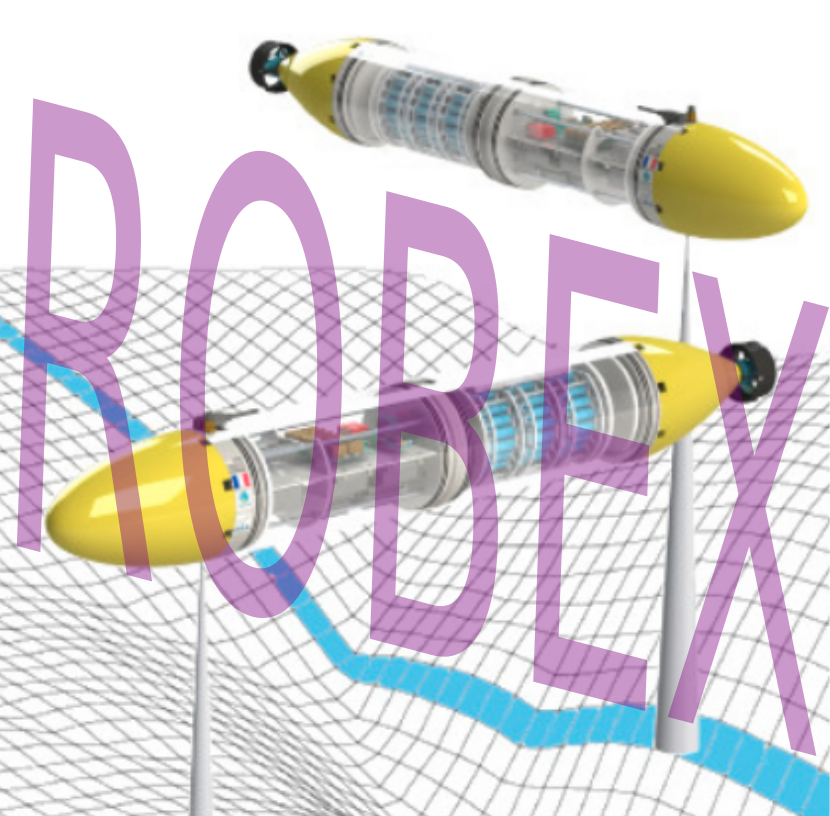
\includegraphics[height=0.6cm]{imgs/logo_robex}}
    \end{tabular}
}

\addtobeamertemplate{frametitle}{}{%
    \begin{tikzpicture}[remember picture,overlay]
    \node[anchor=north east,yshift=2pt] at (current page.north east) {
\includegraphics[height=0.85cm]{imgs/logo_ensta_aid}};
    \end{tikzpicture}
}

\begin{document}

    \maketitle

    % \section{Context}

    %     \begin{frame}{PhD thesis}
    %         \centering
    %         \begin{minipage}[c]{0.58\textwidth}
    %             \begin{block}{Research laboratory}
    %                 \vspace{0.2cm}
    %                 \begin{itemize}
    %                     \item ENSTA Bretagne, UMR 6285, Lab-STICC, IAO, ROBEX
    %                 \end{itemize}
    %             \end{block}

    %             \begin{block}{Supervisiors}
    %                 \begin{itemize}
    %                     \item Luc Jaulin
    %                     \item Fabrice Le Bars
    %                 \end{itemize}
    %             \end{block}

    %             \begin{block}{Funding}
    %                 \begin{itemize}
    %                     \item AID funding: Jean-Daniel Masson
    %                 \end{itemize}
    %             \end{block}
    %         \end{minipage}
    %         \hfill
    %         \begin{minipage}[c]{0.4\textwidth}
    %             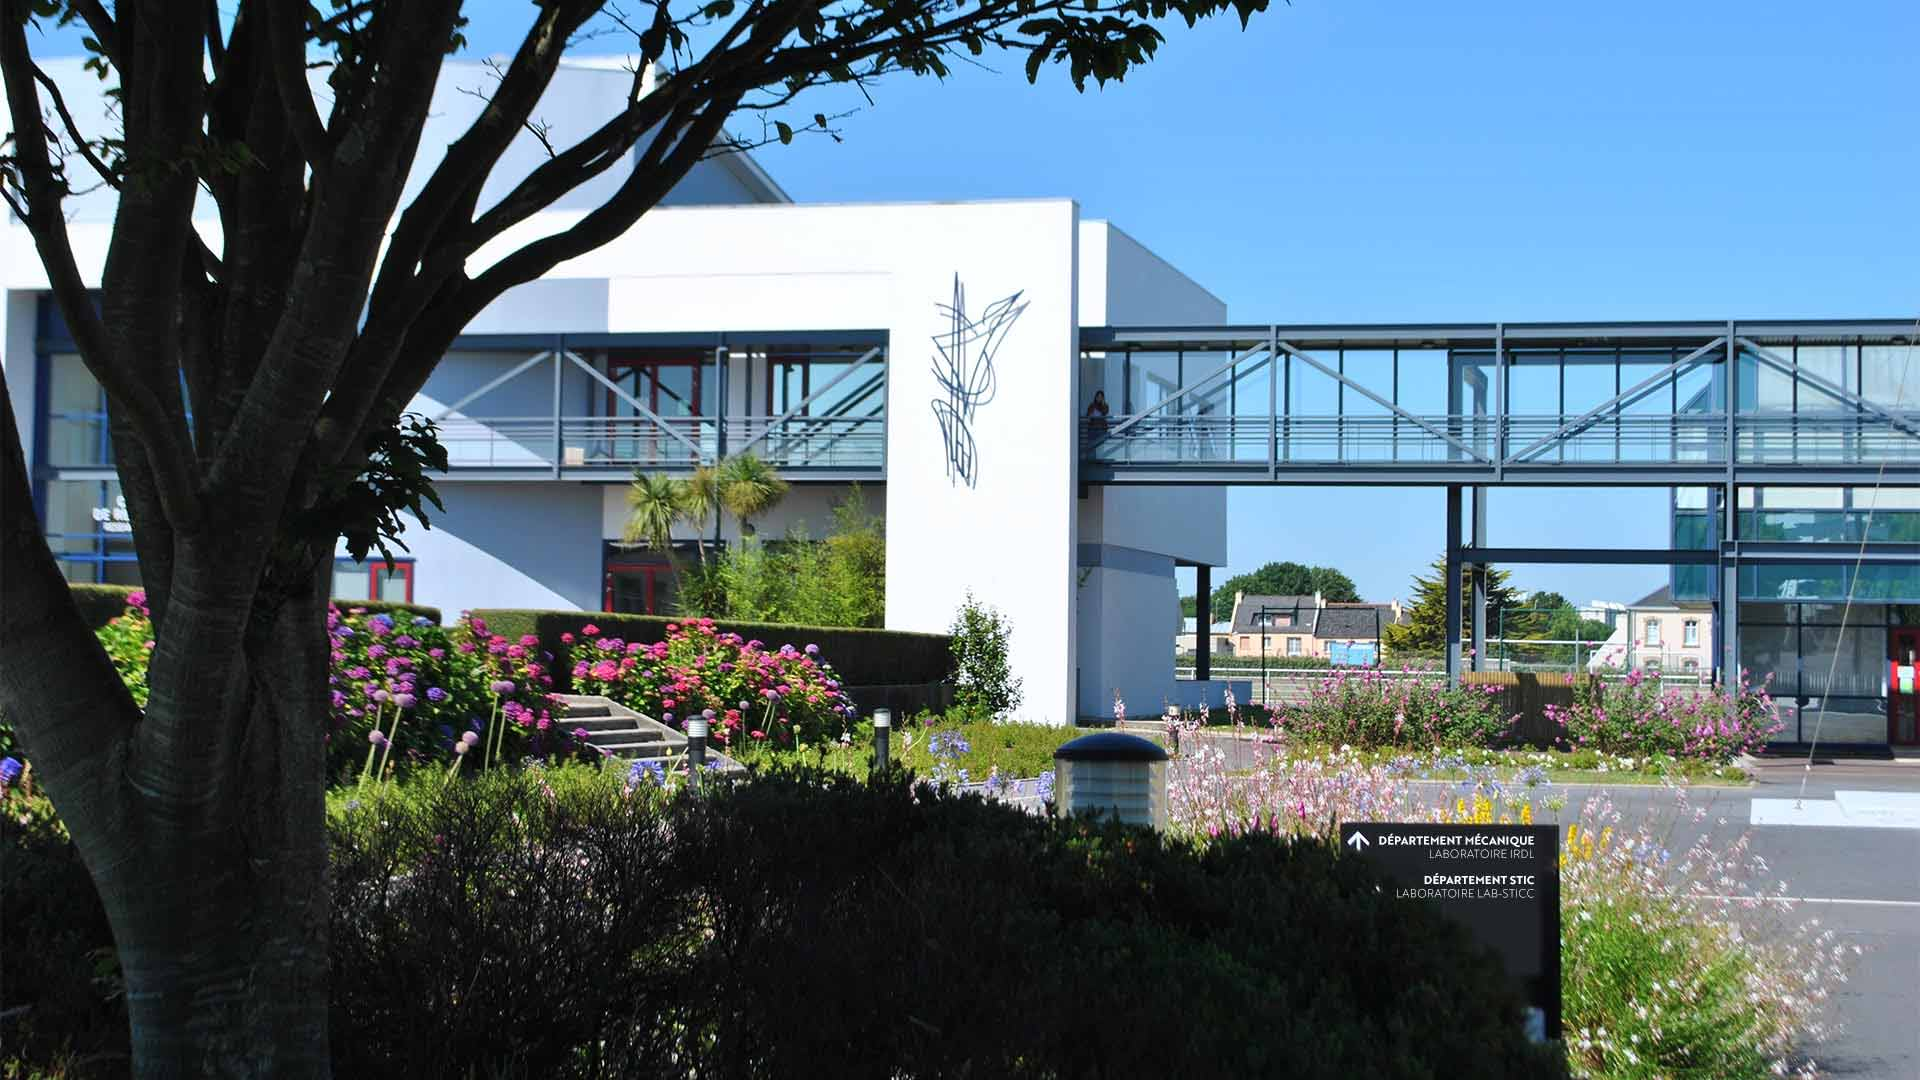
\includegraphics[height=0.7\textheight, trim={24cm 0 16cm 0}, clip]{imgs/ensta.jpg}
    %         \end{minipage}
    %     \end{frame}

    %     \begin{frame}{Goal}
    %         \begin{minipage}[c]{0.55\textwidth}
    %             \begin{block}{AUV}
    %                 \vspace{0.25cm}
    %                 \begin{itemize}
    %                     \item Control of torpedo-like AUV \\ 
    %                     \item Riptide's micro-uuv
    %                 \end{itemize}
    %             \end{block}
    %             \begin{block}{Environment}
    %                 \begin{itemize}
    %                     \item Constrained environment \\ 
    %                     \item Pool, harbor, ...
    %                 \end{itemize}
    %             \end{block}
    %             \begin{block}{Goals}
    %                 \begin{itemize}
    %                     \item Reactivity \\
    %                     \item Manoeuvrability
    %                 \end{itemize}
    %             \end{block}
    %         \end{minipage}
    %         \hfill
    %         \begin{minipage}[c]{0.4\textwidth}
    %             \begin{figure}[htb]
    %                 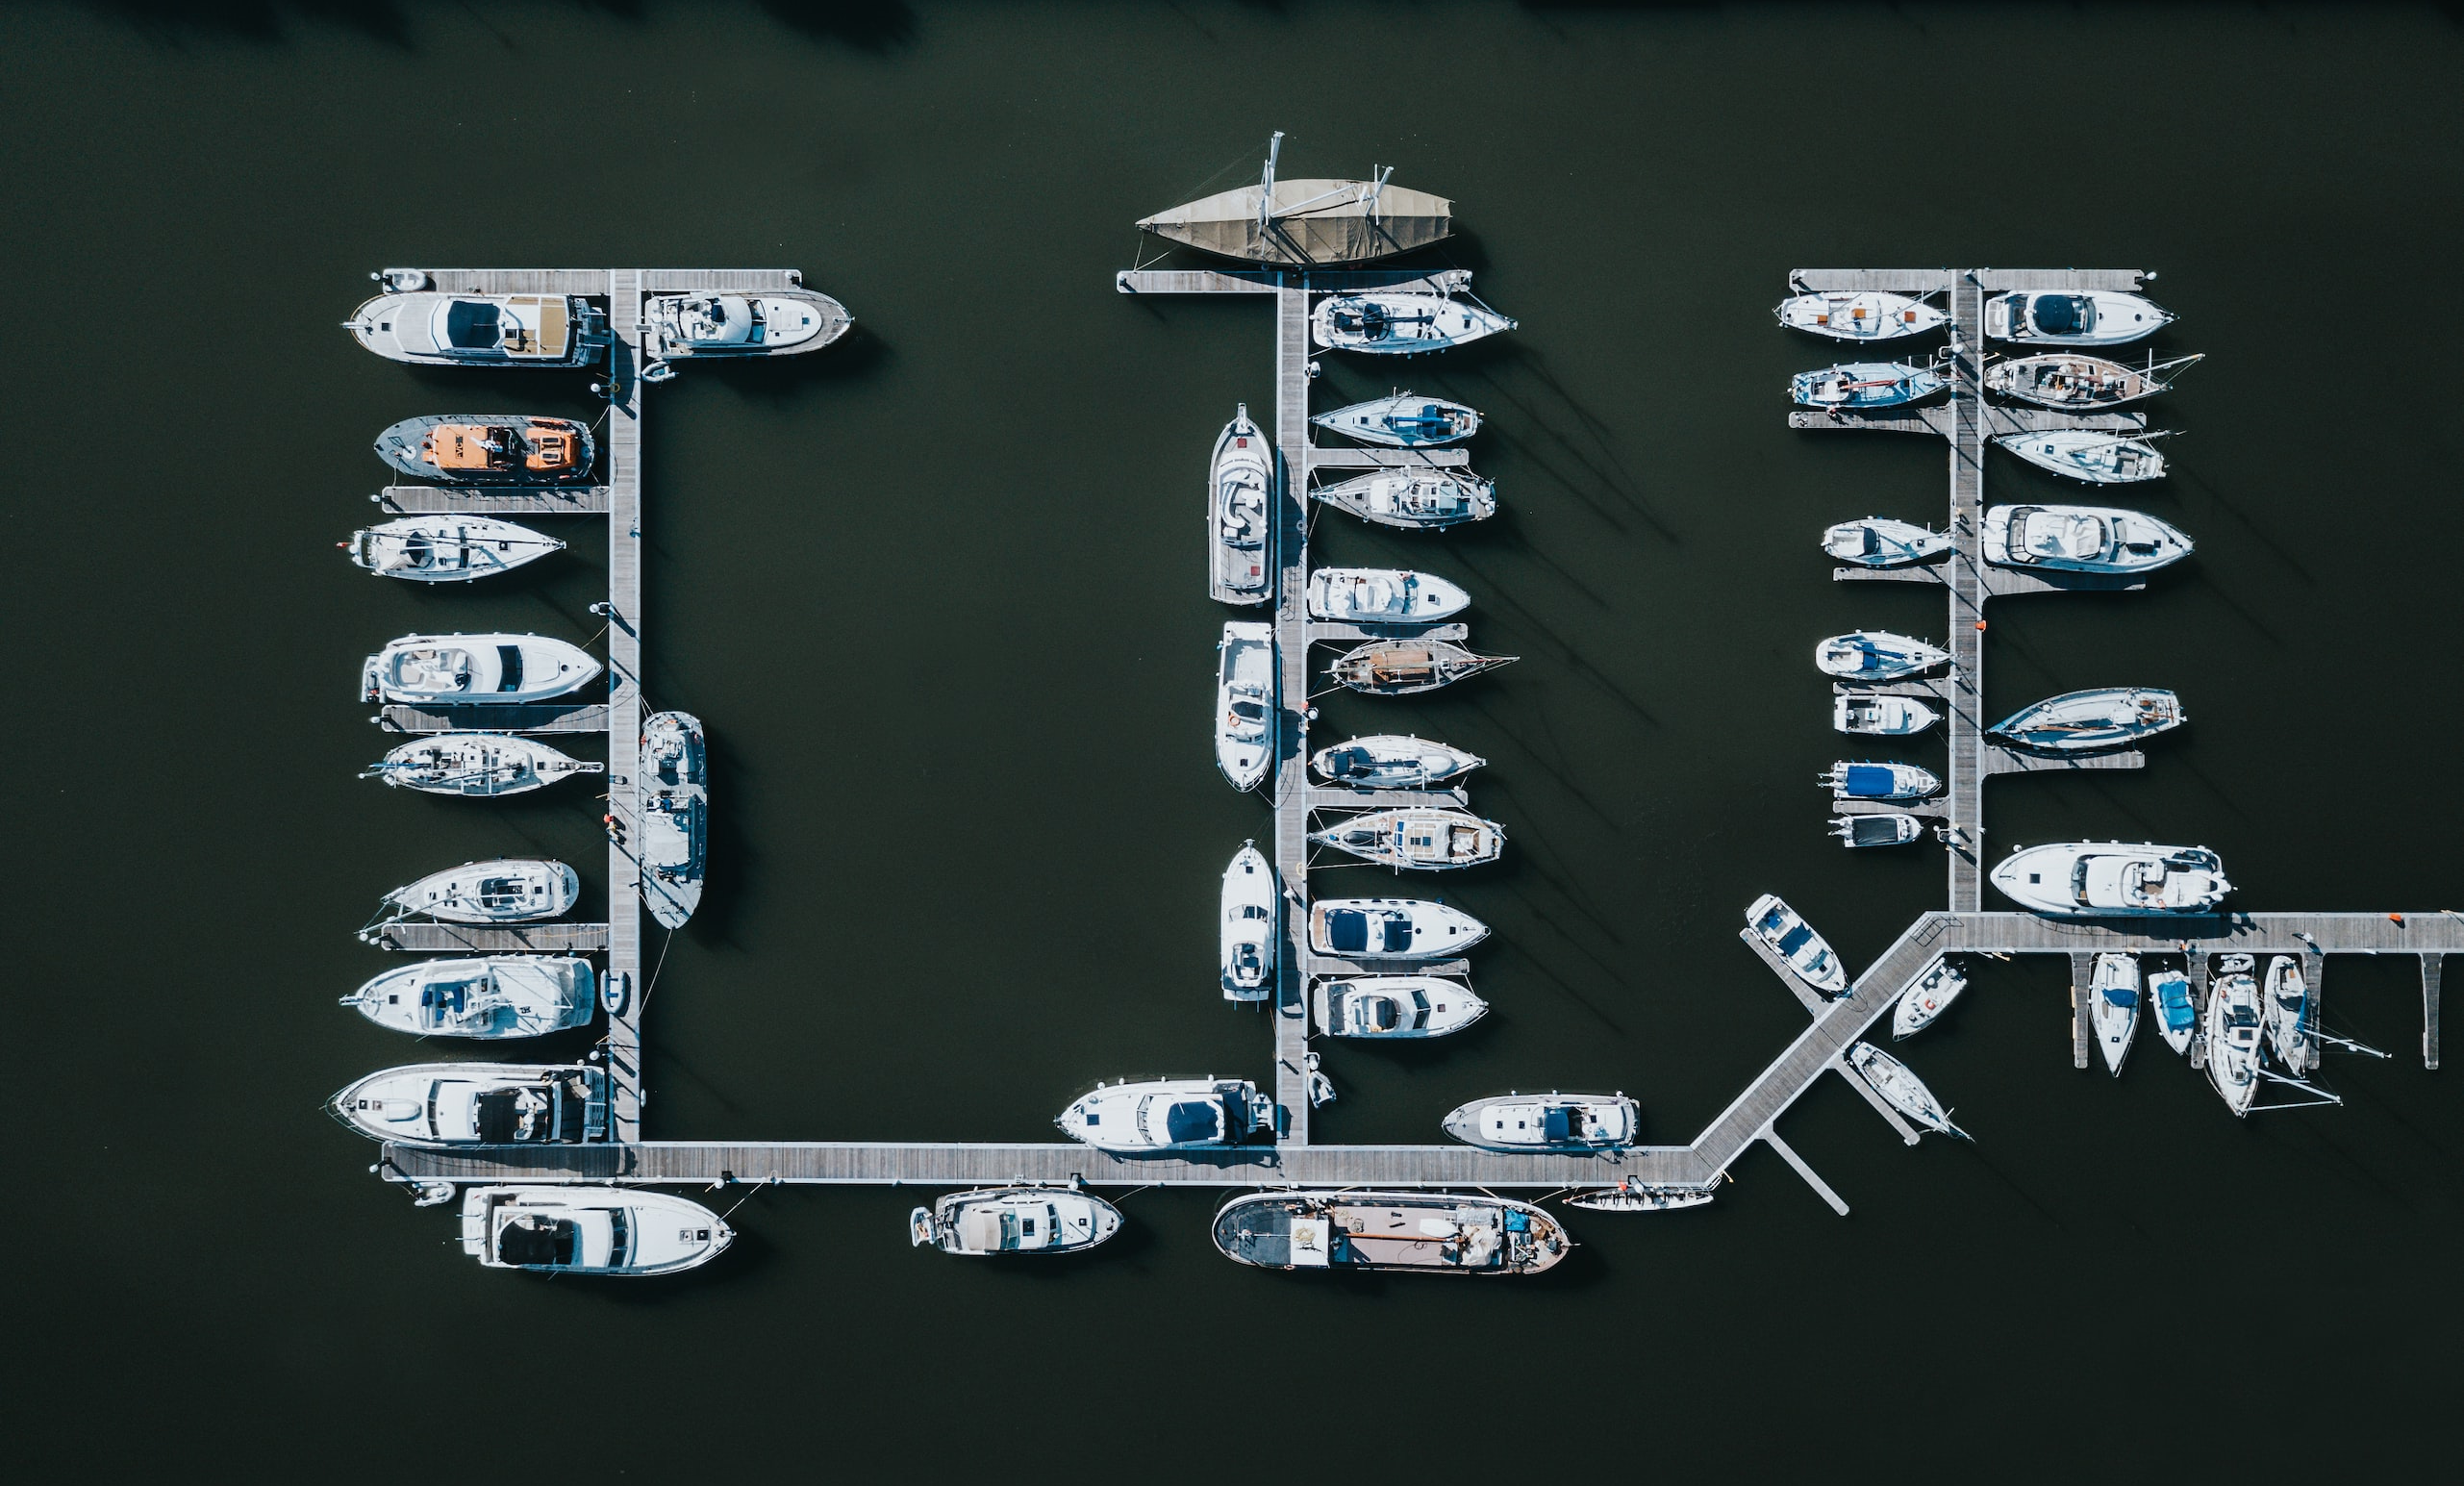
\includegraphics[width=\textwidth]{imgs/harbour.png}

    %                 \vspace{.1cm}

    %                 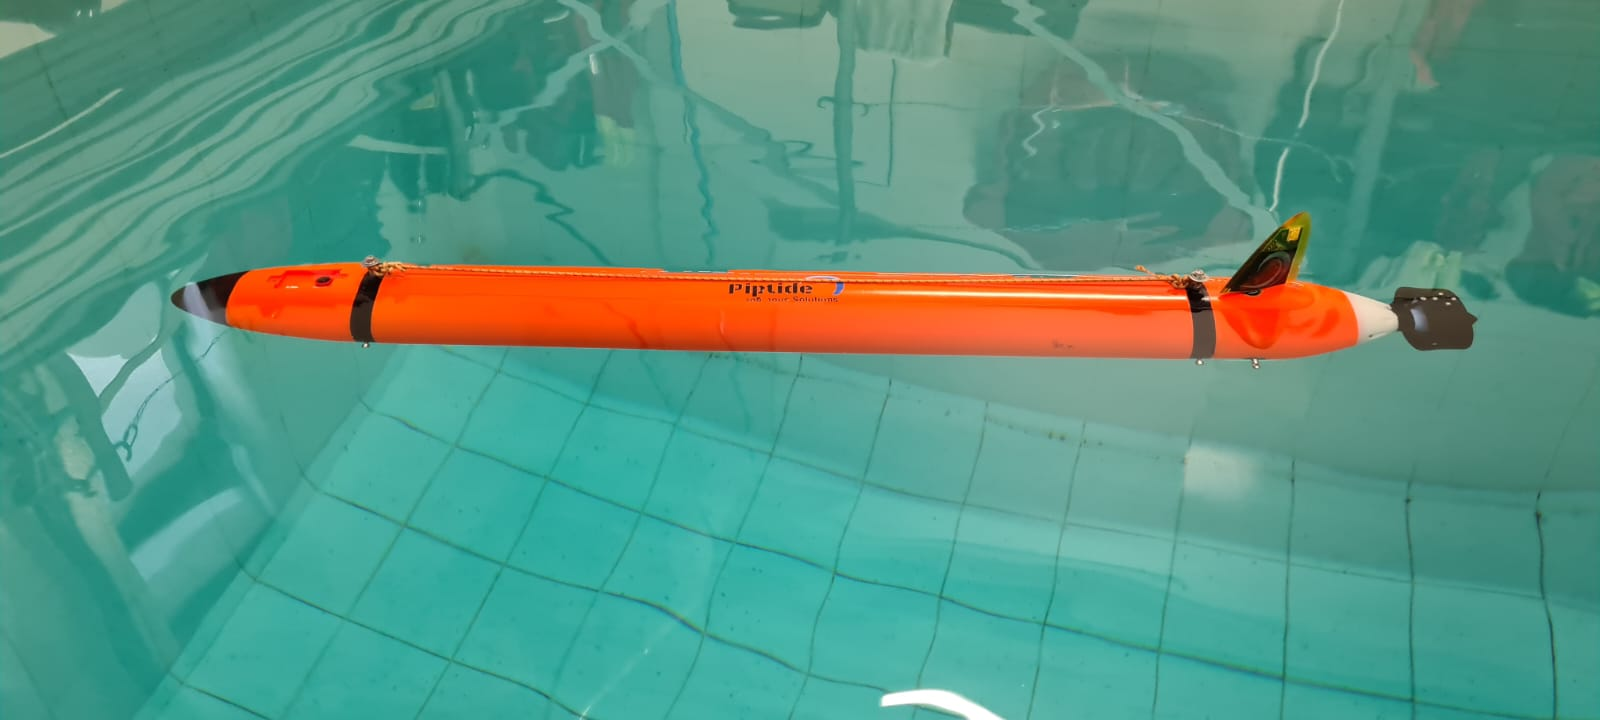
\includegraphics[width=\textwidth]{imgs/Riptide.jpeg}
    %                 \caption{Harbor and Riptide in the ENSTA Bretagne pool}
    %             \end{figure}
    %         \end{minipage}
    %     \end{frame}


        \begin{frame}{Why cycles ?}
            \hfill
            \begin{minipage}[c]{.6\textwidth}
                \begin{block}{Cycles}
                    \vspace{2.5mm}
                    \begin{itemize}
                        \item Omnipresent in wildlife
                        \item Natural mimetism
                        \item Transpose cycles to robotics
                    \end{itemize}
                \end{block}
                \begin{block}{Cycles in robotics}
                    \begin{itemize}
                        \item Frequent with Finite State Machine
                        \item Provides robustness and stability
                    \end{itemize}
                \end{block}
            \end{minipage}
            \hfill
            \begin{minipage}[c]{.35\textwidth}
                \begin{figure}
                    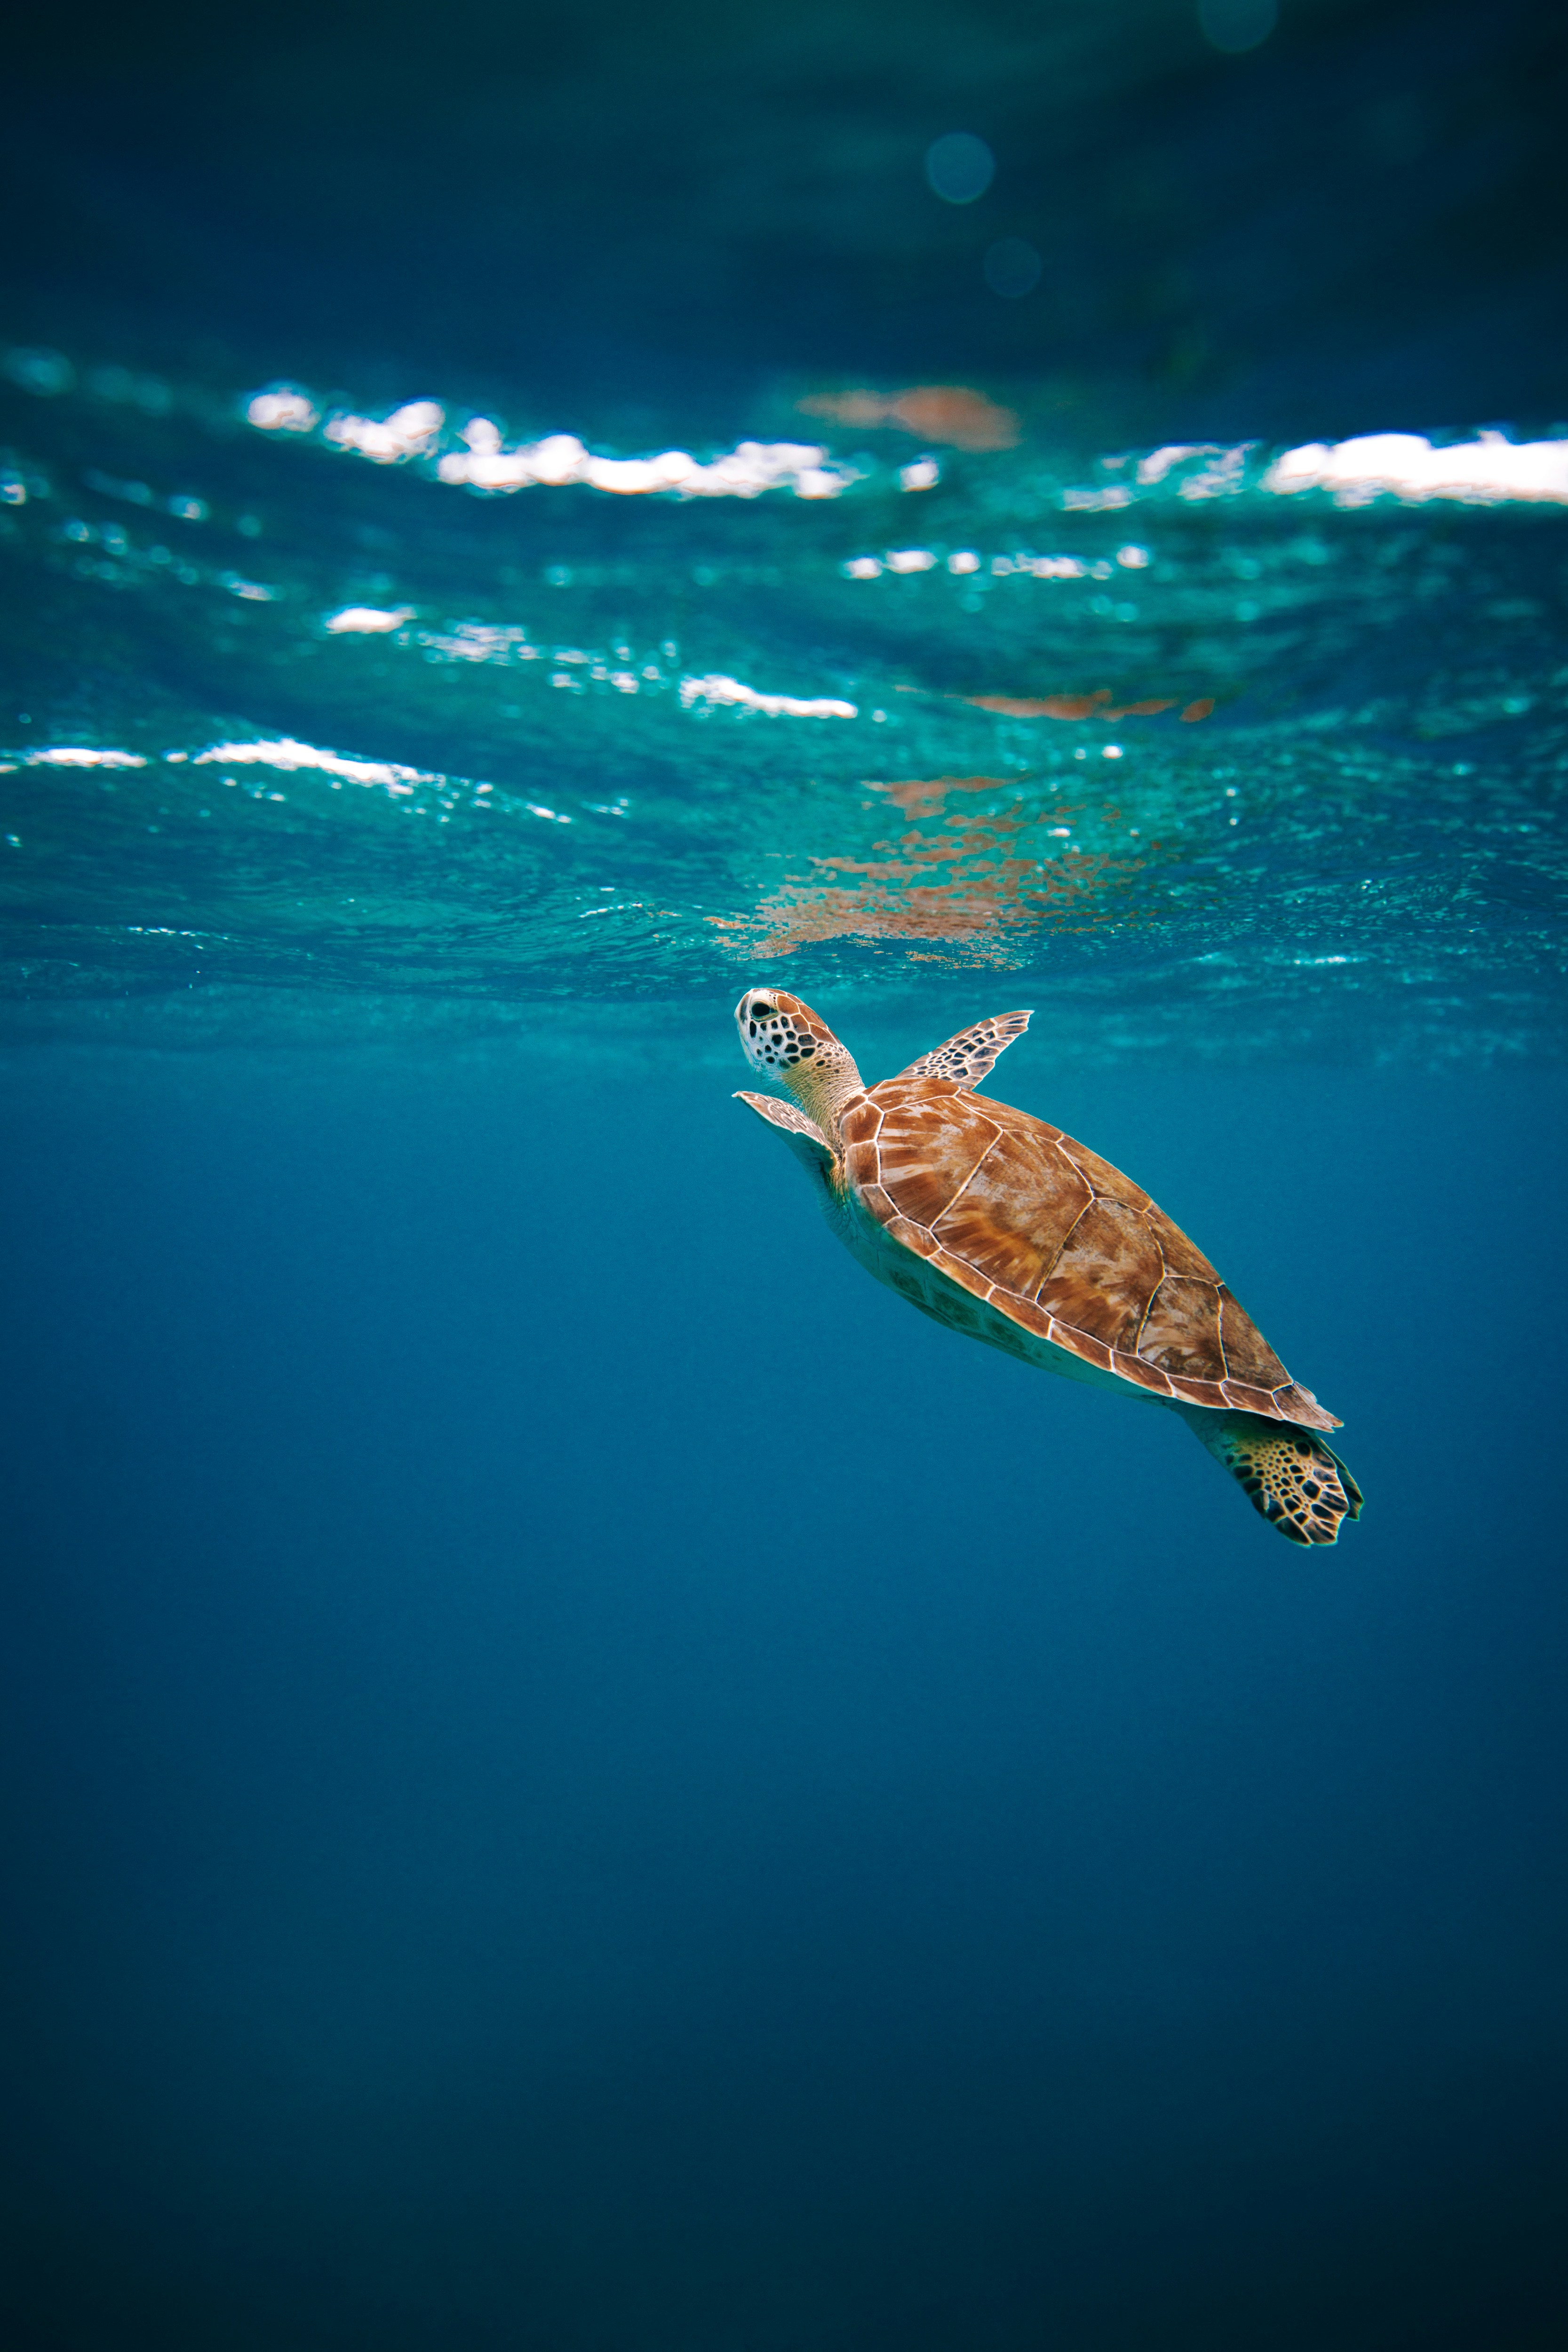
\includegraphics[width=\textwidth]{imgs/turtle.jpg}
                    \caption{Sea turtle are performing cycles}
                \end{figure}
            \end{minipage}
        \end{frame}

    \subsection{Formalism}

        \begin{frame}{Dubins car}
            \centering
            \begin{minipage}{.6\textwidth}
                \begin{block}{Evolution equation}
                    \vspace*{2.5mm}
                    \begin{equation}
                        \dot{\mathbf{x}} = f_r(\mathbf{x}, \mathbf{s}) = 
                        \begin{cases*}
                            \dot{x} = v \cdot \cos(\theta) \\
                            \dot{y} = v \cdot \sin(\theta) \\
                            \dot{\theta} = s
                        \end{cases*}
                    \end{equation}
                \end{block}
            \end{minipage}
            \hfill
            \begin{minipage}{.38\textwidth}
                \begin{figure}
                    \begin{overprint}
                        \onslide<1>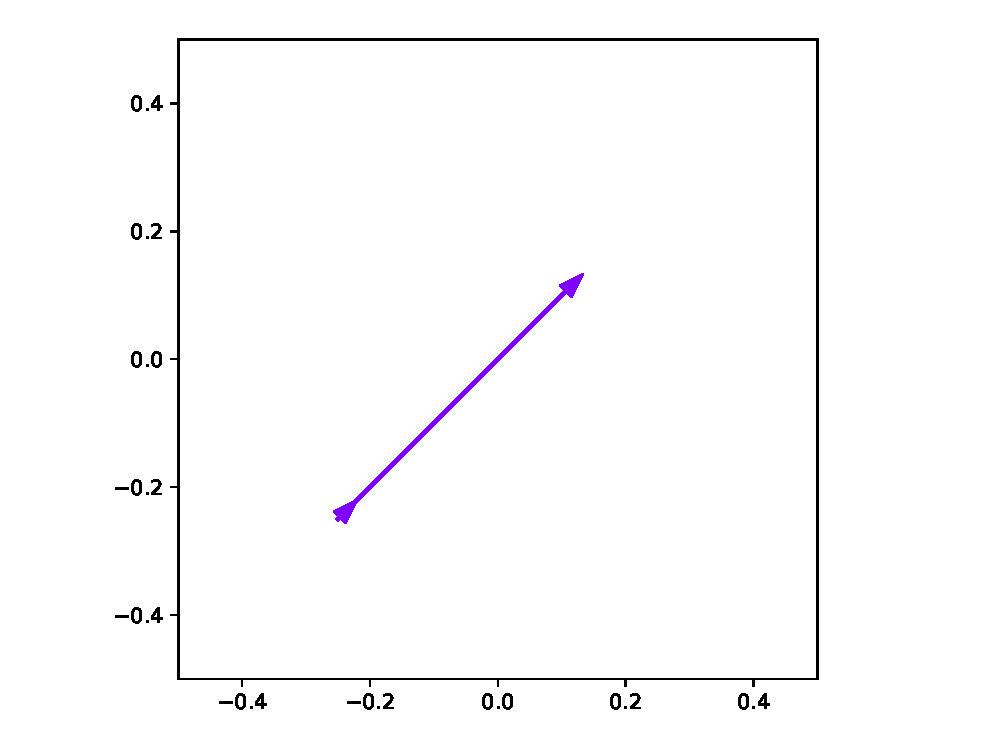
\includegraphics[width=\textwidth]{imgs/dubins_straight}
                        \onslide<2>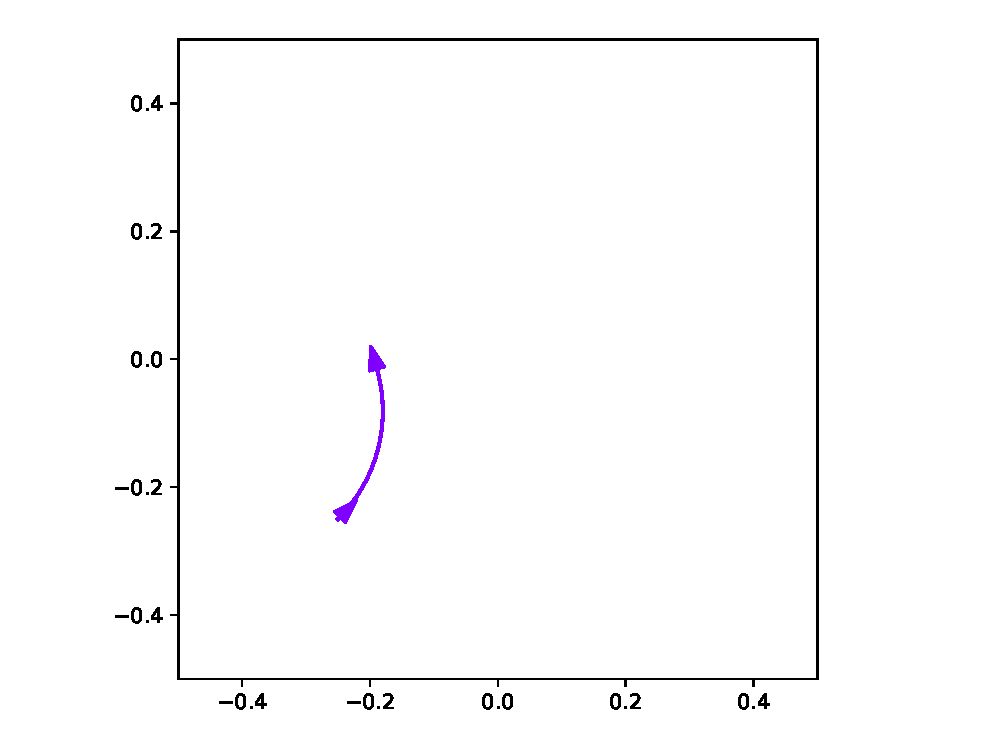
\includegraphics[width=\textwidth]{imgs/dubins_left}
                        \onslide<3>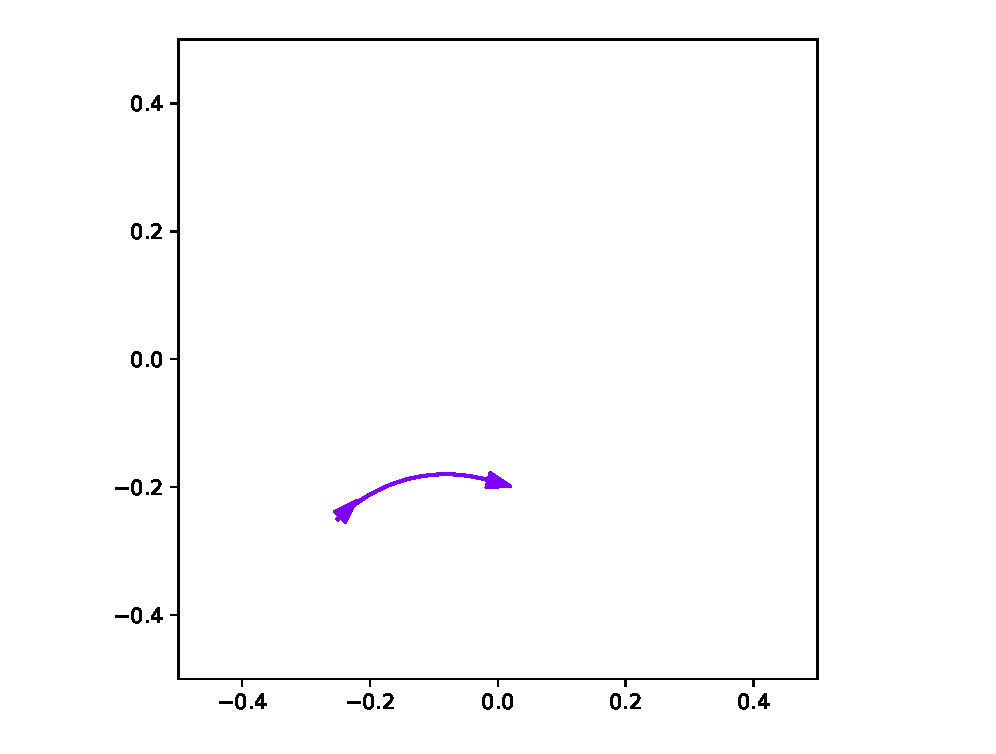
\includegraphics[width=\textwidth]{imgs/dubins_right}
                    \end{overprint}
                    \caption{Dubins car}
                \end{figure}
            \end{minipage}

            \begin{block}{Steering input}
                \begin{itemize}[<+->]
                    \item s = 0: the car goes straight forward
                    \item s = 1: the car turns counter-clockwise
                    \item s = -1: the car turns clockwise
                \end{itemize}
            \end{block}
        \end{frame}

        \begin{frame}{Timed automaton}
            \centering
            
            \begin{minipage}[c]{.5\textwidth}
                \begin{figure}
                    \resizebox{\textwidth}{!}{
                    \begin{tikzpicture}[shorten >=1pt,on grid,auto]
    
                        \node[state,initial,accepting] (q_0) at (180: 2cm) {$s=0$};
                        \foreach \a in {1,...,5}{
                            \pgfmathtruncatemacro{\b}{mod(\a,2)};            
                            \node[state] (q_\a) at (-\a*360/6+180: 2cm) {$s=\b$};
                        }
                
                        \foreach \a in {0,1,...,5}{
                            \pgfmathtruncatemacro{\b}{mod(\a+1,6)};
                            % Put in RubineRed the first transition
                            \draw[->,>=latex] (q_\a) edge[bend left=20]
                                node[sloped,midway,yshift=-.82em]{$|$}
                                node[midway,sloped,{\ifnum\a<3 above\else below\fi},font=\bfseries, alt=<2->{color={\ifnum\a<3 RubineRed\else black\fi}}]
                                {\alt<2->{\ifnum\a<3 $d_\a+\mathbf{u_\a}$\else $d_\a$\fi}{$d_\a$}}
                                (q_\b);
                        }
                    \end{tikzpicture}}
                    \caption{Timed automaton}
                \end{figure} 
            \end{minipage}\
            \hfill
            \begin{minipage}[c]{.45\textwidth}
                \begin{figure}
                    \begin{overprint}
                        \onslide<1-2>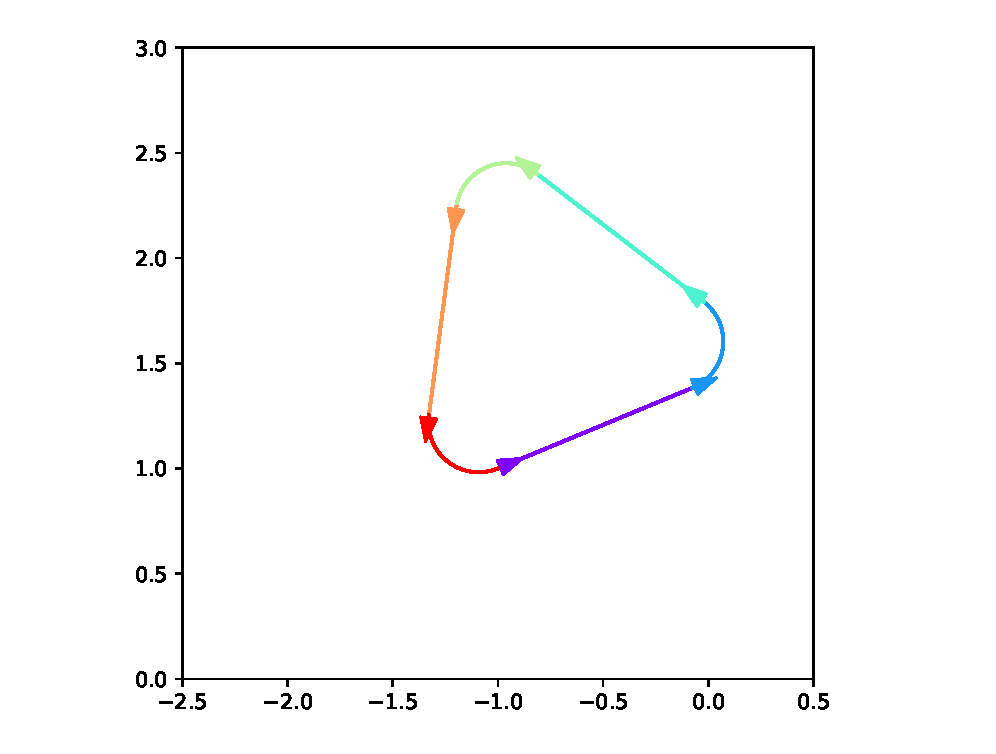
\includegraphics[width=\textwidth]{imgs/robot_cycle}
                        \onslide<3>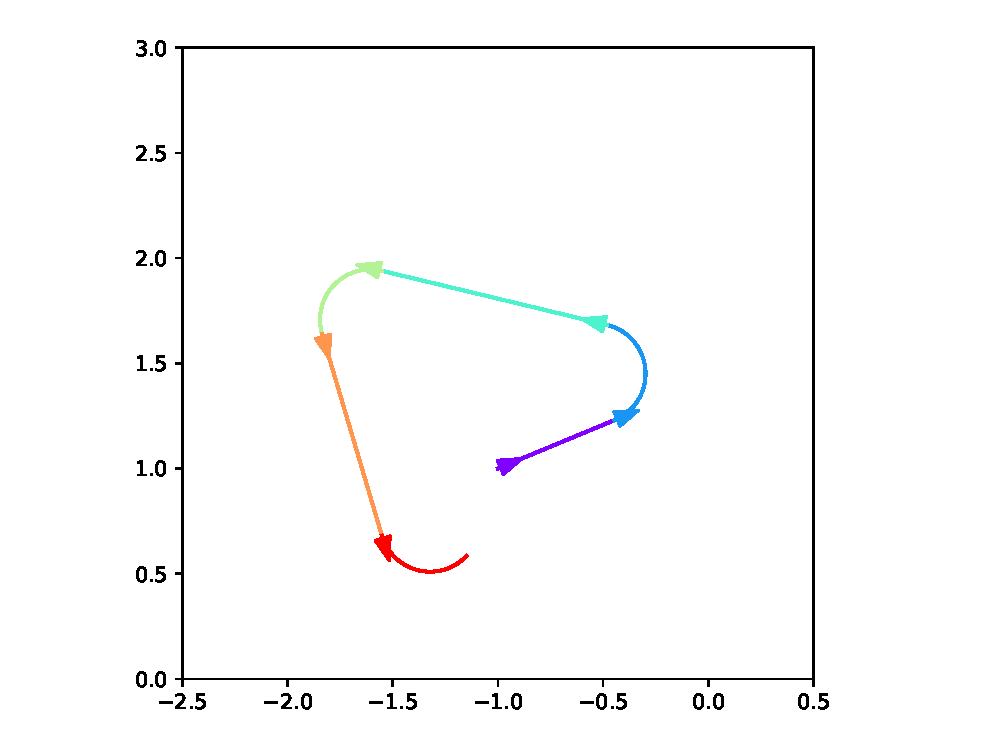
\includegraphics[width=\textwidth]{imgs/robot_cycle_u}
                        \onslide<4>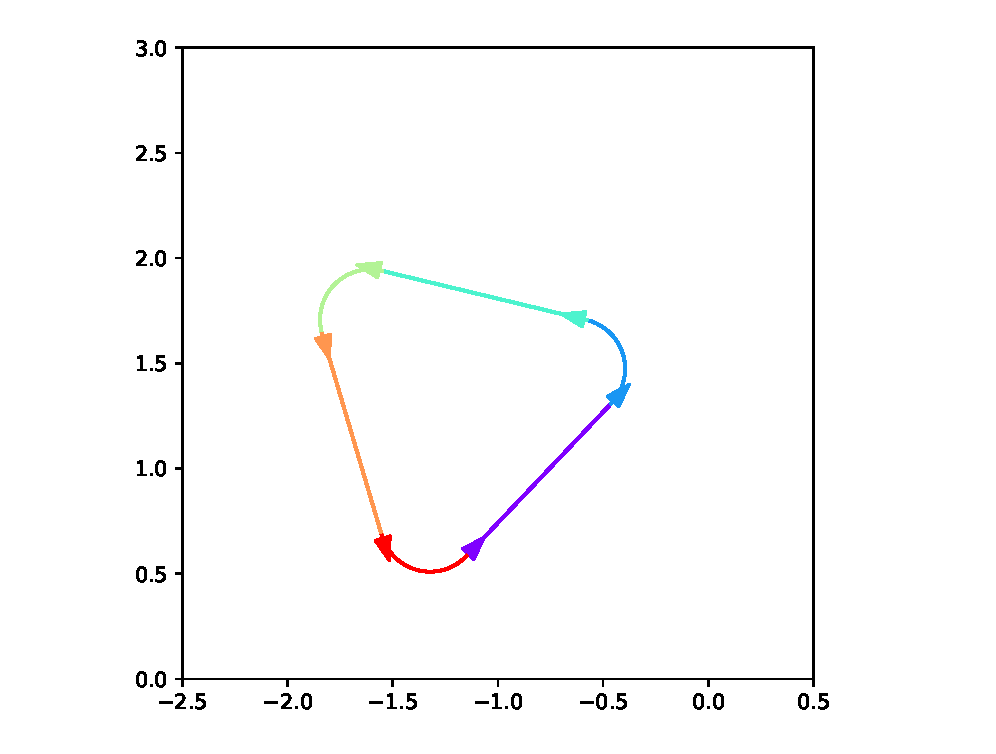
\includegraphics[width=\textwidth]{imgs/robot_cycle_next}
                    \end{overprint}
                    \caption{Robot trajectory}
                \end{figure}
            \end{minipage}
            \begin{minipage}{.85\textwidth}
                \begin{block}<2->{Control of the cycle}
                    \vspace{2.5mm}
                    \begin{overprint}
                        \onslide<2>$$\mathbf{x_0} = \begin{bmatrix}-1& 1& \frac{\pi}{8}\end{bmatrix} \qquad \mathbf{u_0} = \begin{bmatrix}0& 0& 0\end{bmatrix}^T$$
                        \onslide<3>$$\mathbf{x_1} = \begin{bmatrix}-1& 1& \frac{\pi}{8}\end{bmatrix} \qquad \mathbf{u_1} = \begin{bmatrix}-0.4& 0.2& 0.1\end{bmatrix}^T$$
                        \onslide<4>$$\mathbf{x_2} = \begin{bmatrix}-1.15& 0.58& 0.81\end{bmatrix} \qquad \mathbf{u_2} = \begin{bmatrix}0& 0& 0\end{bmatrix}^T$$
                    \end{overprint}
                \end{block}
            \end{minipage}
        \end{frame}

        \begin{frame}{Measurements}
            \begin{minipage}{.48\textwidth}
                \begin{block}{Map}
                    \vspace{2.5mm}
                    \begin{itemize}
                        \item Triangle room
                    \end{itemize}
                \end{block}
                \begin{block}{Measurements}
                    \begin{itemize}
                        \item Sonar ranging measurements
                        \item Distance to the walls
                        \item 3 Measurements per cycle
                    \end{itemize}
                \end{block}
            \end{minipage}
            \hfill
            \begin{minipage}{.48\textwidth}
                \begin{figure}
                    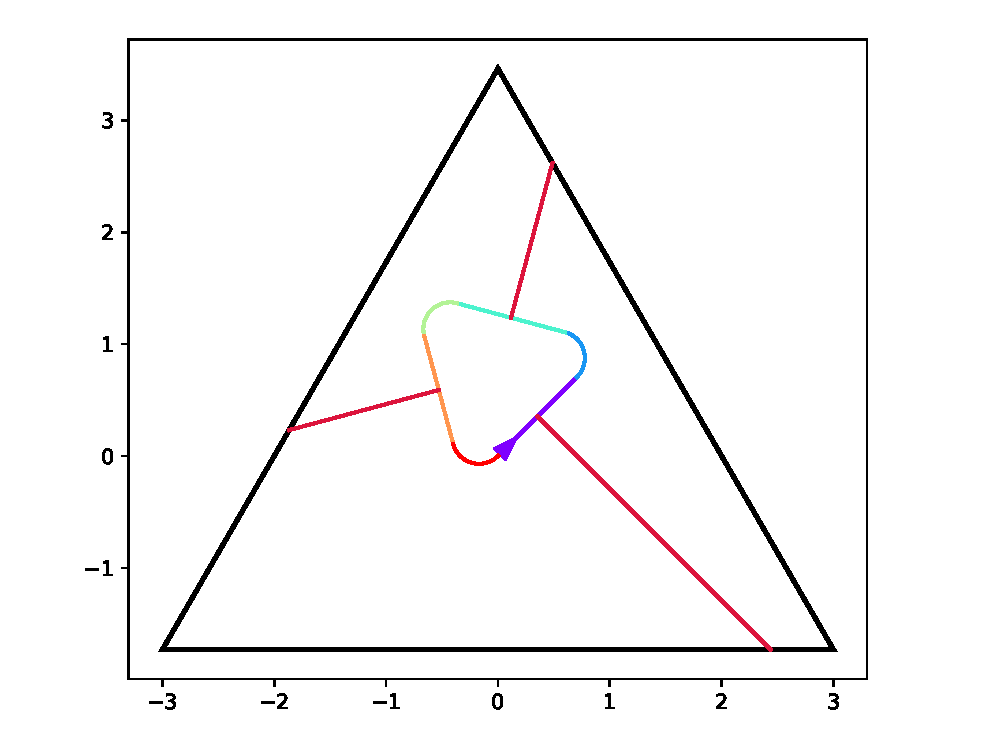
\includegraphics[width=\textwidth]{imgs/cycle_measurements}
                    \caption{Map and measurements taken during the cycle}
                \end{figure}
            \end{minipage}
        \end{frame}

        \begin{frame}{Control of cycle}
            \begin{minipage}{.48\textwidth}
                \begin{block}{Discrete system}
                    \begin{eqnarray}
                        \mathbf{x}_{k+1} &=& f(\mathbf{x}_k, \mathbf{u}_k)\\
                        \mathbf{y}_k &=& g(\mathbf{x}_k, \mathbf{u}_k)
                    \end{eqnarray}
                \end{block}
                \begin{block}{Operating point}
                    \begin{align}
                        \bar{\mathbf{x}} &= [0,\ 0,\ 0]^T\\
                        \bar{\mathbf{u}} &= [0,\ 0,\ 0]^T
                    \end{align}
                \end{block}
            \end{minipage}
            \hfill
            \begin{minipage}{.48\textwidth}
                \begin{block}{Polarization}
                    \begin{align}
                        \tilde{\mathbf{x}} &= \mathbf{x} - \bar{\mathbf{x}}\\
                        \tilde{\mathbf{u}} &= \mathbf{u} - \bar{\mathbf{u}}
                    \end{align}
                \end{block}
                \begin{block}{Linearization}
                    \begin{eqnarray}
                        \tilde{\mathbf{x}_{k+1}} &= A\tilde{\mathbf{x}_k} + B\tilde{\mathbf{u}_k}\\
                        \tilde{\mathbf{y}_k} &= C\tilde{\mathbf{x}_k} + D\tilde{\mathbf{u}_k}
                    \end{eqnarray}
                \end{block}
            
            \end{minipage}
        \end{frame}

        \begin{frame}{Linear control of non-linear systems}
            \begin{minipage}{.5\textwidth}
                \begin{block}{Stability approach}
                    \vspace{2.5mm}
                    \begin{itemize}
                        \item Luenberger state observer
                        \item Linear controller on polarized system
                    \end{itemize}
                \end{block}
                \begin{block}{Regulator tuning}
                    \begin{itemize}
                        \item Pole placement method inside the unit circle
                        \item Poles of L: $[0.15, 0.15, 0.15]$
                        \item Poles of K: $[0.6, 0.6, 0.6]$
                    \end{itemize}
                \end{block}
            \end{minipage}
            \hfill
            \begin{minipage}{.45\textwidth}
                \begin{figure}
                    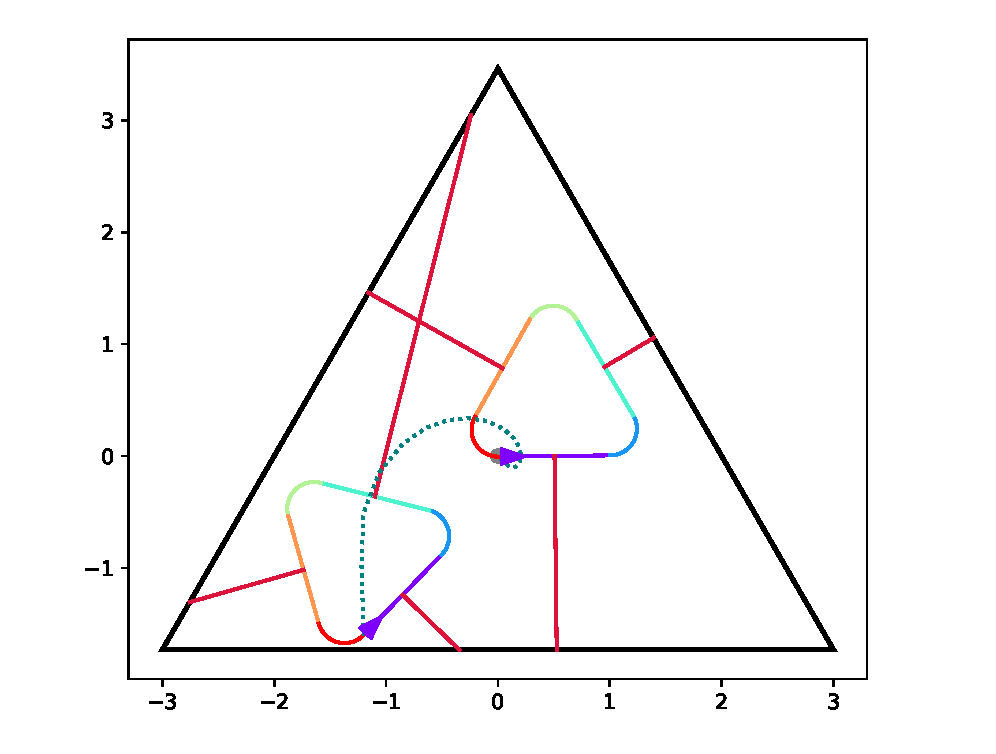
\includegraphics[width=\textwidth]{imgs/cycle_regulation}
                    \caption{Regulation of the cycle around the operating point}
                \end{figure}
            \end{minipage}
        \end{frame}

        \begin{frame}{Results}
            \centering
            \begin{minipage}{.65\textwidth}
                \begin{figure}
                    \begin{subfigure}{.48\textwidth}
                        \centering
                        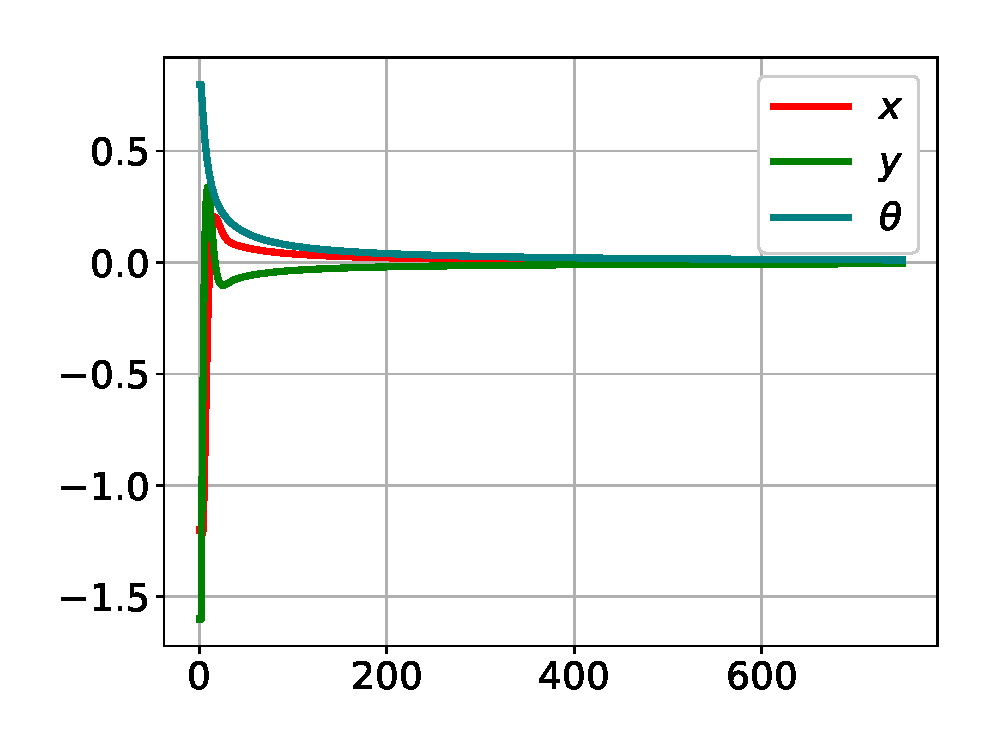
\includegraphics[width=\textwidth]{imgs/state}
                        \caption{State}
                    \end{subfigure}
                    \begin{subfigure}{.48\textwidth}
                        \centering
                        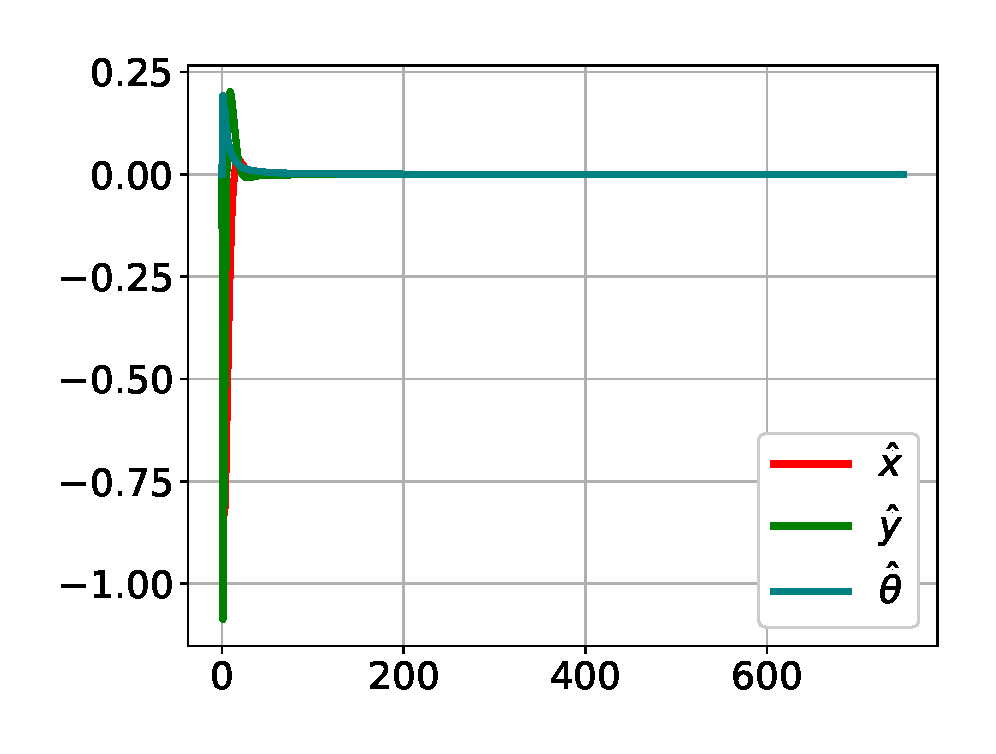
\includegraphics[width=\textwidth]{imgs/estimated_state}
                        \caption{Estimated state}
                    \end{subfigure}
                    \begin{subfigure}{.48\textwidth}
                        \centering
                        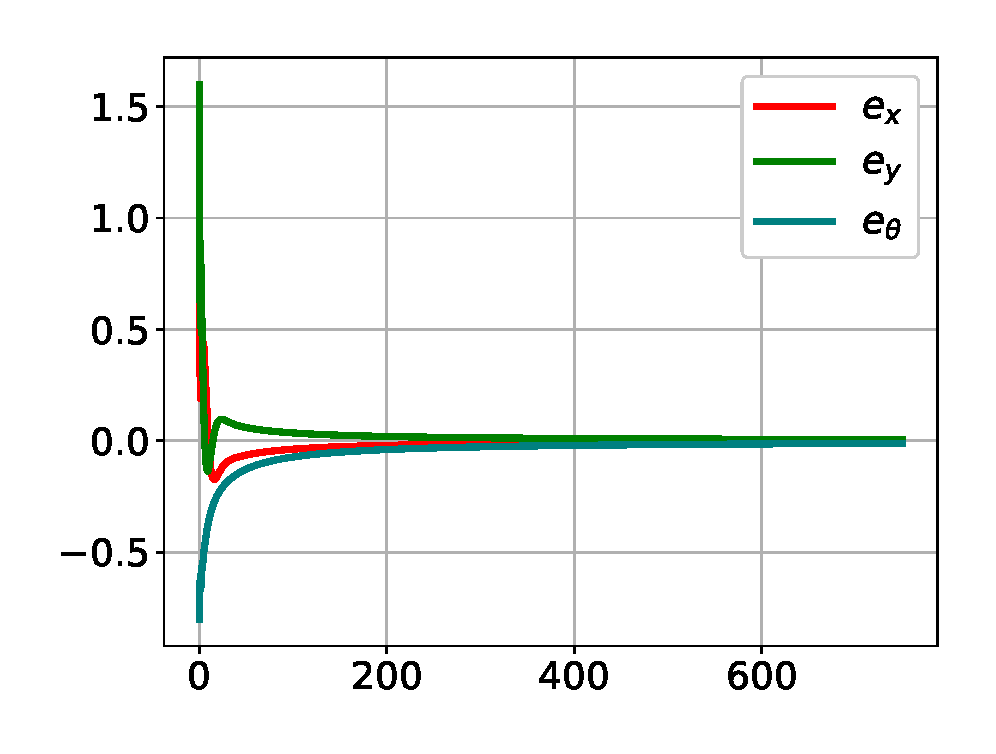
\includegraphics[width=\textwidth]{imgs/error}
                        \caption{Error}
                    \end{subfigure}
                    \begin{subfigure}{.48\textwidth}
                        \centering
                        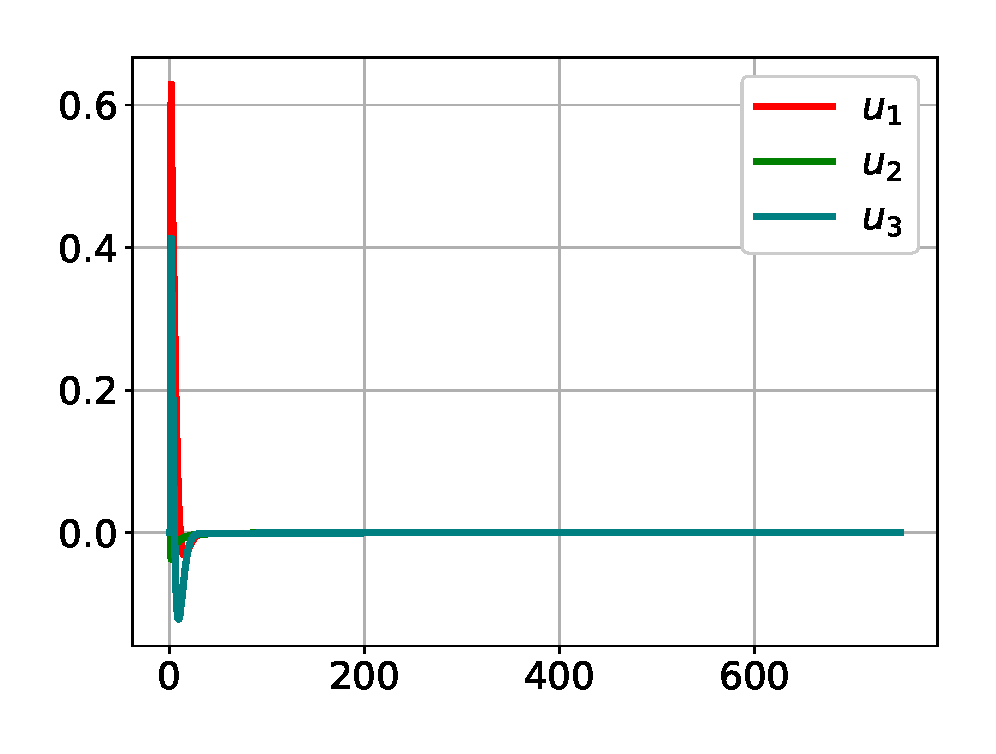
\includegraphics[width=\textwidth]{imgs/control}
                        \caption{Control}
                    \end{subfigure}
                    \caption{Simulation results}
                \end{figure}
            \end{minipage}
        \end{frame}

        \begin{frame}{Conclusion \& Outlook}
            \centering
            \begin{minipage}[c]{.6\textwidth}
                \begin{block}{Conclusion}
                    \vspace{2.5mm}
                    \begin{itemize}
                        \item Control a cycle
                        \item Classical stability approach
                        \item Converging behavior
                    \end{itemize}
                \end{block}
                \begin{block}{Problem statement}
                    \begin{itemize}
                        \item Observability: 3 measurements
                        \item Interval: 2 measurements
                        \item Trial on torpedo-like AUV able to turn inside pool
                    \end{itemize}
                \end{block}
            \end{minipage}
            \hfill
            \begin{minipage}[c]{.35\textwidth}
                \begin{figure}
                    \begin{subfigure}{\textwidth}
                        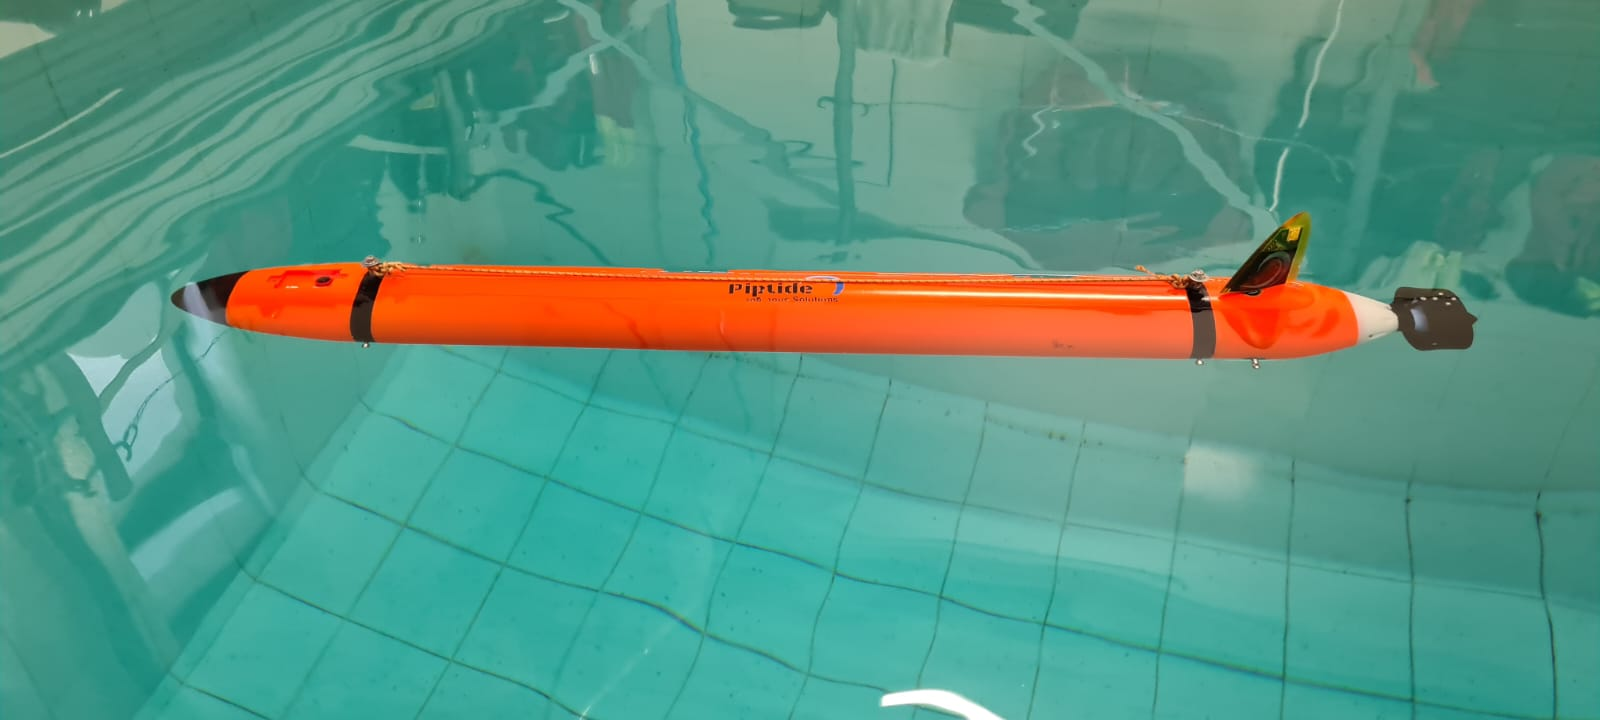
\includegraphics[width=\textwidth]{imgs/Riptide}
                        \caption{Riptide (2023 Colorized)}
                    \end{subfigure}
                    \begin{subfigure}{\textwidth}
                        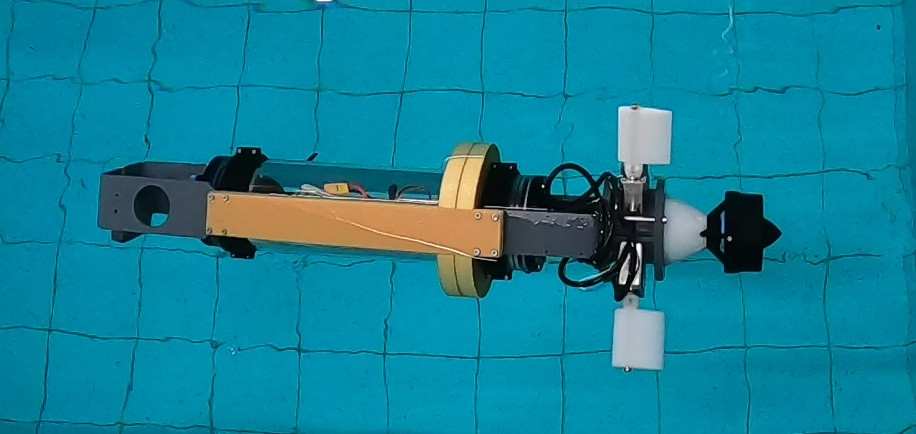
\includegraphics[width=\textwidth]{imgs/MAUV}
                        \caption{MAUV}
                    \end{subfigure}
                    \caption{Robots in ENSTA Bretagne pool}
                \end{figure}
            \end{minipage}
        \end{frame}

        \appendix

        \begin{frame}[standout]
            Questions?
        \end{frame}

        \maketitle

\end{document}